\chapter{Architektur}

Um die Anwendung modular und damit auch erweiterbar zu halten, haben wir uns bei der Umsetzung des Projektes am MVC-Prinziep orientiert. Deshalb lässt sich die gesammte Anwendung in drei Komponenten aufteilen: Das Model ist für die Repräsentation und Speicherung der Daten zuständig. Diese Daten werden im View angezeigt. Er beinhaltet in der Hauptsache die Layouts der verschiedenen Activities sowie die zugehörigen Code-Behind-Klassen. Der Controller ist für die Verarbeitung der Daten zuständigt und stellt somit das Bindeglied zwischen Model und View dar. 

Eine grafische Übersicht über die hier vorgestellte Architektur ist in Abbildung~\ref{fig:arcdia} zu sehen.
\begin{landscape}
\begin{figure}[htpb]
	\centering
	\scalebox{0.75}{% Graphic for TeX using PGF
% Title: /home/tobias/Documents/Studium/android/projekt/documentation/content/02_architektur_diagramm.dia
% Creator: Dia v0.97.3
% CreationDate: Sun Nov 29 21:08:29 2015
% For: tobias
% \usepackage{tikz}
% The following commands are not supported in PSTricks at present
% We define them conditionally, so when they are implemented,
% this pgf file will use them.
\ifx\du\undefined
  \newlength{\du}
\fi
\setlength{\du}{15\unitlength}
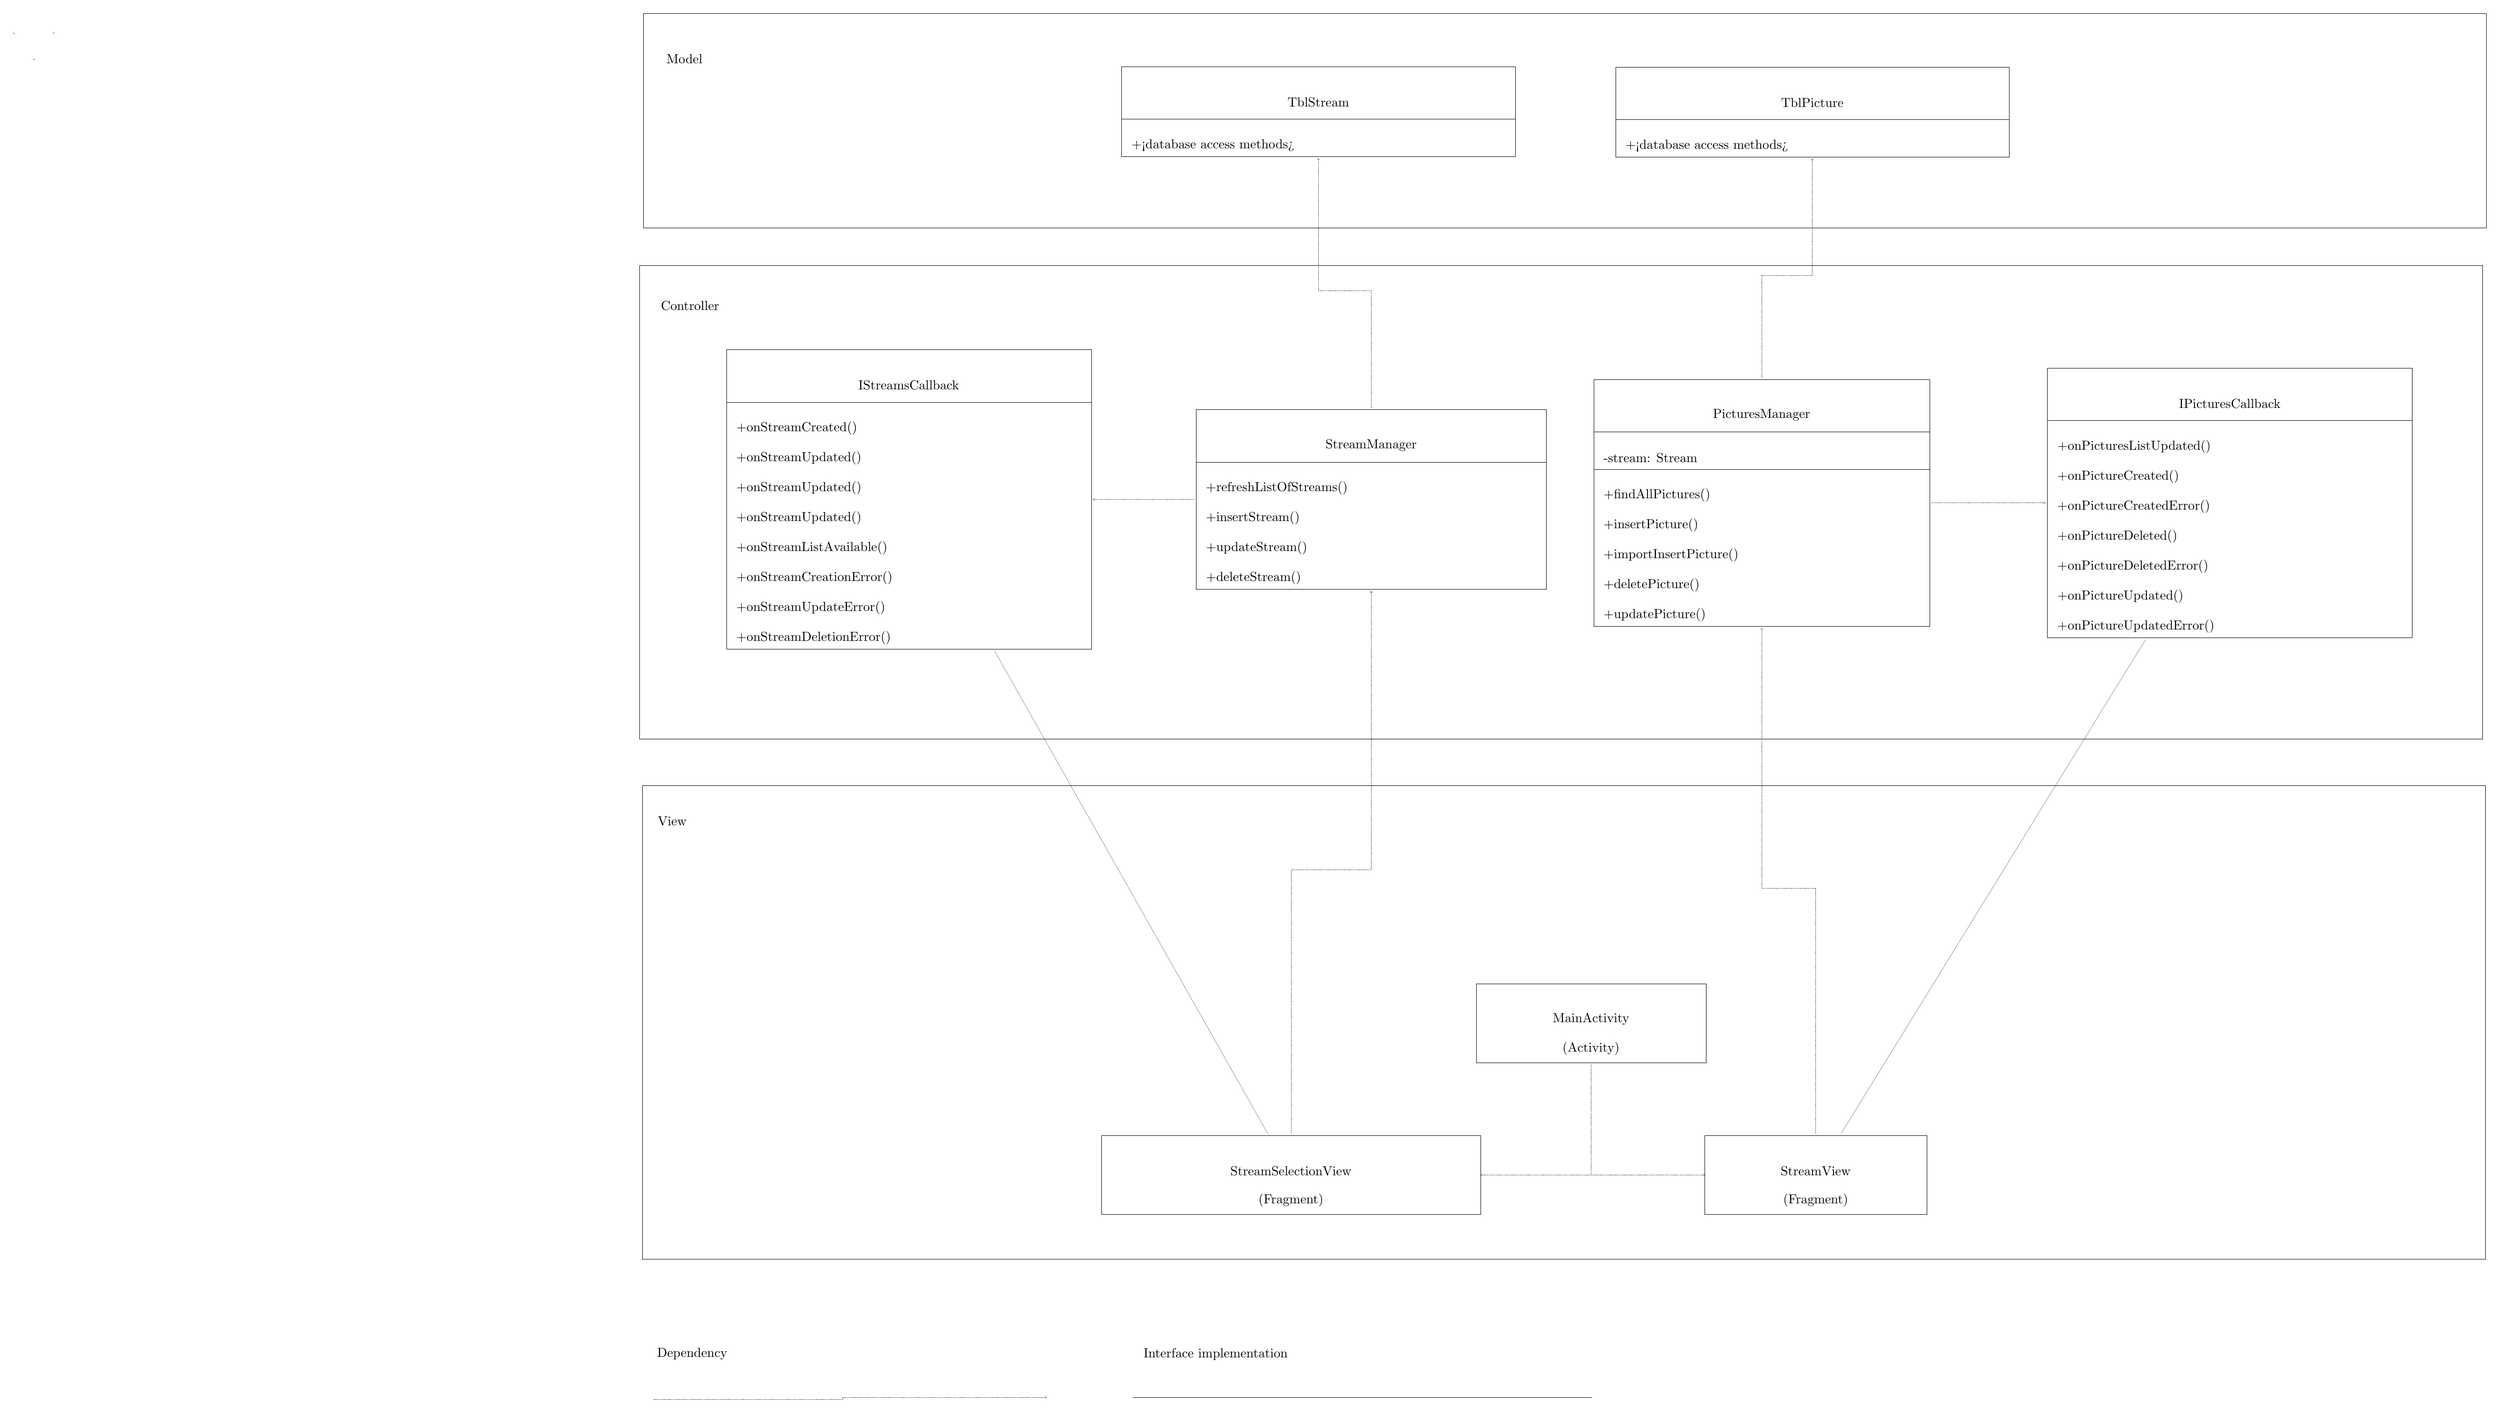
\begin{tikzpicture}
\pgftransformxscale{1.000000}
\pgftransformyscale{-1.000000}
\definecolor{dialinecolor}{rgb}{0.000000, 0.000000, 0.000000}
\pgfsetstrokecolor{dialinecolor}
\definecolor{dialinecolor}{rgb}{1.000000, 1.000000, 1.000000}
\pgfsetfillcolor{dialinecolor}
\pgfsetlinewidth{0.100000\du}
\pgfsetdash{}{0pt}
\pgfsetdash{}{0pt}
\pgfsetmiterjoin
\definecolor{dialinecolor}{rgb}{0.000000, 0.000000, 0.000000}
\pgfsetstrokecolor{dialinecolor}
\draw (17.735000\du,20.700000\du)--(17.735000\du,33.350000\du)--(66.935000\du,33.350000\du)--(66.935000\du,20.700000\du)--cycle;
\pgfsetlinewidth{0.100000\du}
\pgfsetdash{}{0pt}
\pgfsetdash{}{0pt}
\pgfsetmiterjoin
\definecolor{dialinecolor}{rgb}{0.000000, 0.000000, 0.000000}
\pgfsetstrokecolor{dialinecolor}
\draw (17.670000\du,6.810000\du)--(17.670000\du,19.460000\du)--(66.870000\du,19.460000\du)--(66.870000\du,6.810000\du)--cycle;
\pgfsetlinewidth{0.100000\du}
\pgfsetdash{}{0pt}
\definecolor{dialinecolor}{rgb}{1.000000, 1.000000, 1.000000}
\pgfsetfillcolor{dialinecolor}
\fill (30.000000\du,30.050000\du)--(30.000000\du,32.150000\du)--(40.117500\du,32.150000\du)--(40.117500\du,30.050000\du)--cycle;
\definecolor{dialinecolor}{rgb}{0.000000, 0.000000, 0.000000}
\pgfsetstrokecolor{dialinecolor}
\draw (30.000000\du,30.050000\du)--(30.000000\du,32.150000\du)--(40.117500\du,32.150000\du)--(40.117500\du,30.050000\du)--cycle;
% setfont left to latex
\definecolor{dialinecolor}{rgb}{0.000000, 0.000000, 0.000000}
\pgfsetstrokecolor{dialinecolor}
\node at (35.058750\du,31.000000\du){StreamSelectionView};
% setfont left to latex
\definecolor{dialinecolor}{rgb}{0.000000, 0.000000, 0.000000}
\pgfsetstrokecolor{dialinecolor}
\node at (35.058750\du,31.775000\du){(Fragment)};
\pgfsetlinewidth{0.100000\du}
\pgfsetdash{}{0pt}
\definecolor{dialinecolor}{rgb}{1.000000, 1.000000, 1.000000}
\pgfsetfillcolor{dialinecolor}
\fill (46.100000\du,30.050000\du)--(46.100000\du,32.150000\du)--(52.030000\du,32.150000\du)--(52.030000\du,30.050000\du)--cycle;
\definecolor{dialinecolor}{rgb}{0.000000, 0.000000, 0.000000}
\pgfsetstrokecolor{dialinecolor}
\draw (46.100000\du,30.050000\du)--(46.100000\du,32.150000\du)--(52.030000\du,32.150000\du)--(52.030000\du,30.050000\du)--cycle;
% setfont left to latex
\definecolor{dialinecolor}{rgb}{0.000000, 0.000000, 0.000000}
\pgfsetstrokecolor{dialinecolor}
\node at (49.065000\du,31.000000\du){StreamView};
% setfont left to latex
\definecolor{dialinecolor}{rgb}{0.000000, 0.000000, 0.000000}
\pgfsetstrokecolor{dialinecolor}
\node at (49.065000\du,31.775000\du){(Fragment)};
\pgfsetlinewidth{0.100000\du}
\pgfsetdash{}{0pt}
\definecolor{dialinecolor}{rgb}{1.000000, 1.000000, 1.000000}
\pgfsetfillcolor{dialinecolor}
\fill (40.000000\du,26.000000\du)--(40.000000\du,28.100000\du)--(46.135000\du,28.100000\du)--(46.135000\du,26.000000\du)--cycle;
\definecolor{dialinecolor}{rgb}{0.000000, 0.000000, 0.000000}
\pgfsetstrokecolor{dialinecolor}
\draw (40.000000\du,26.000000\du)--(40.000000\du,28.100000\du)--(46.135000\du,28.100000\du)--(46.135000\du,26.000000\du)--cycle;
% setfont left to latex
\definecolor{dialinecolor}{rgb}{0.000000, 0.000000, 0.000000}
\pgfsetstrokecolor{dialinecolor}
\node at (43.067500\du,26.950000\du){MainActivity};
% setfont left to latex
\definecolor{dialinecolor}{rgb}{0.000000, 0.000000, 0.000000}
\pgfsetstrokecolor{dialinecolor}
\node at (43.067500\du,27.725000\du){(Activity)};
\pgfsetlinewidth{0.100000\du}
\pgfsetdash{}{0pt}
\definecolor{dialinecolor}{rgb}{1.000000, 1.000000, 1.000000}
\pgfsetfillcolor{dialinecolor}
\fill (55.250000\du,9.550000\du)--(55.250000\du,10.950000\du)--(64.990000\du,10.950000\du)--(64.990000\du,9.550000\du)--cycle;
\definecolor{dialinecolor}{rgb}{0.000000, 0.000000, 0.000000}
\pgfsetstrokecolor{dialinecolor}
\draw (55.250000\du,9.550000\du)--(55.250000\du,10.950000\du)--(64.990000\du,10.950000\du)--(64.990000\du,9.550000\du)--cycle;
% setfont left to latex
\definecolor{dialinecolor}{rgb}{0.000000, 0.000000, 0.000000}
\pgfsetstrokecolor{dialinecolor}
\node at (60.120000\du,10.500000\du){IPicturesCallback};
\definecolor{dialinecolor}{rgb}{1.000000, 1.000000, 1.000000}
\pgfsetfillcolor{dialinecolor}
\fill (55.250000\du,10.950000\du)--(55.250000\du,16.750000\du)--(64.990000\du,16.750000\du)--(64.990000\du,10.950000\du)--cycle;
\definecolor{dialinecolor}{rgb}{0.000000, 0.000000, 0.000000}
\pgfsetstrokecolor{dialinecolor}
\draw (55.250000\du,10.950000\du)--(55.250000\du,16.750000\du)--(64.990000\du,16.750000\du)--(64.990000\du,10.950000\du)--cycle;
% setfont left to latex
\definecolor{dialinecolor}{rgb}{0.000000, 0.000000, 0.000000}
\pgfsetstrokecolor{dialinecolor}
\node[anchor=west] at (55.400000\du,11.650000\du){+onPicturesListUpdated()};
% setfont left to latex
\definecolor{dialinecolor}{rgb}{0.000000, 0.000000, 0.000000}
\pgfsetstrokecolor{dialinecolor}
\node[anchor=west] at (55.400000\du,12.450000\du){+onPictureCreated()};
% setfont left to latex
\definecolor{dialinecolor}{rgb}{0.000000, 0.000000, 0.000000}
\pgfsetstrokecolor{dialinecolor}
\node[anchor=west] at (55.400000\du,13.250000\du){+onPictureCreatedError()};
% setfont left to latex
\definecolor{dialinecolor}{rgb}{0.000000, 0.000000, 0.000000}
\pgfsetstrokecolor{dialinecolor}
\node[anchor=west] at (55.400000\du,14.050000\du){+onPictureDeleted()};
% setfont left to latex
\definecolor{dialinecolor}{rgb}{0.000000, 0.000000, 0.000000}
\pgfsetstrokecolor{dialinecolor}
\node[anchor=west] at (55.400000\du,14.850000\du){+onPictureDeletedError()};
% setfont left to latex
\definecolor{dialinecolor}{rgb}{0.000000, 0.000000, 0.000000}
\pgfsetstrokecolor{dialinecolor}
\node[anchor=west] at (55.400000\du,15.650000\du){+onPictureUpdated()};
% setfont left to latex
\definecolor{dialinecolor}{rgb}{0.000000, 0.000000, 0.000000}
\pgfsetstrokecolor{dialinecolor}
\node[anchor=west] at (55.400000\du,16.450000\du){+onPictureUpdatedError()};
\pgfsetlinewidth{0.100000\du}
\pgfsetdash{}{0pt}
\definecolor{dialinecolor}{rgb}{1.000000, 1.000000, 1.000000}
\pgfsetfillcolor{dialinecolor}
\fill (19.985000\du,9.060000\du)--(19.985000\du,10.460000\du)--(29.725000\du,10.460000\du)--(29.725000\du,9.060000\du)--cycle;
\definecolor{dialinecolor}{rgb}{0.000000, 0.000000, 0.000000}
\pgfsetstrokecolor{dialinecolor}
\draw (19.985000\du,9.060000\du)--(19.985000\du,10.460000\du)--(29.725000\du,10.460000\du)--(29.725000\du,9.060000\du)--cycle;
% setfont left to latex
\definecolor{dialinecolor}{rgb}{0.000000, 0.000000, 0.000000}
\pgfsetstrokecolor{dialinecolor}
\node at (24.855000\du,10.010000\du){IStreamsCallback};
\definecolor{dialinecolor}{rgb}{1.000000, 1.000000, 1.000000}
\pgfsetfillcolor{dialinecolor}
\fill (19.985000\du,10.460000\du)--(19.985000\du,17.060000\du)--(29.725000\du,17.060000\du)--(29.725000\du,10.460000\du)--cycle;
\definecolor{dialinecolor}{rgb}{0.000000, 0.000000, 0.000000}
\pgfsetstrokecolor{dialinecolor}
\draw (19.985000\du,10.460000\du)--(19.985000\du,17.060000\du)--(29.725000\du,17.060000\du)--(29.725000\du,10.460000\du)--cycle;
% setfont left to latex
\definecolor{dialinecolor}{rgb}{0.000000, 0.000000, 0.000000}
\pgfsetstrokecolor{dialinecolor}
\node[anchor=west] at (20.135000\du,11.160000\du){+onStreamCreated()};
% setfont left to latex
\definecolor{dialinecolor}{rgb}{0.000000, 0.000000, 0.000000}
\pgfsetstrokecolor{dialinecolor}
\node[anchor=west] at (20.135000\du,11.960000\du){+onStreamUpdated()};
% setfont left to latex
\definecolor{dialinecolor}{rgb}{0.000000, 0.000000, 0.000000}
\pgfsetstrokecolor{dialinecolor}
\node[anchor=west] at (20.135000\du,12.760000\du){+onStreamUpdated()};
% setfont left to latex
\definecolor{dialinecolor}{rgb}{0.000000, 0.000000, 0.000000}
\pgfsetstrokecolor{dialinecolor}
\node[anchor=west] at (20.135000\du,13.560000\du){+onStreamUpdated()};
% setfont left to latex
\definecolor{dialinecolor}{rgb}{0.000000, 0.000000, 0.000000}
\pgfsetstrokecolor{dialinecolor}
\node[anchor=west] at (20.135000\du,14.360000\du){+onStreamListAvailable()};
% setfont left to latex
\definecolor{dialinecolor}{rgb}{0.000000, 0.000000, 0.000000}
\pgfsetstrokecolor{dialinecolor}
\node[anchor=west] at (20.135000\du,15.160000\du){+onStreamCreationError()};
% setfont left to latex
\definecolor{dialinecolor}{rgb}{0.000000, 0.000000, 0.000000}
\pgfsetstrokecolor{dialinecolor}
\node[anchor=west] at (20.135000\du,15.960000\du){+onStreamUpdateError()};
% setfont left to latex
\definecolor{dialinecolor}{rgb}{0.000000, 0.000000, 0.000000}
\pgfsetstrokecolor{dialinecolor}
\node[anchor=west] at (20.135000\du,16.760000\du){+onStreamDeletionError()};
\pgfsetlinewidth{0.100000\du}
\pgfsetdash{}{0pt}
\pgfsetbuttcap
\definecolor{dialinecolor}{rgb}{0.000000, 0.000000, 0.000000}
\pgfsetstrokecolor{dialinecolor}
\draw (34.436430\du,29.999752\du)--(27.145924\du,17.110302\du);
\definecolor{dialinecolor}{rgb}{1.000000, 1.000000, 1.000000}
\pgfsetfillcolor{dialinecolor}
\pgfpathellipse{\pgfpoint{27.318236\du}{17.414946\du}}{\pgfpoint{0.350000\du}{0\du}}{\pgfpoint{0\du}{0.350000\du}}
\pgfusepath{fill}
\definecolor{dialinecolor}{rgb}{0.000000, 0.000000, 0.000000}
\pgfsetstrokecolor{dialinecolor}
\pgfpathellipse{\pgfpoint{27.318236\du}{17.414946\du}}{\pgfpoint{0.350000\du}{0\du}}{\pgfpoint{0\du}{0.350000\du}}
\pgfusepath{stroke}
% setfont left to latex
\pgfsetlinewidth{0.100000\du}
\pgfsetdash{}{0pt}
\pgfsetbuttcap
\definecolor{dialinecolor}{rgb}{0.000000, 0.000000, 0.000000}
\pgfsetstrokecolor{dialinecolor}
\draw (49.742611\du,29.999763\du)--(57.873104\du,16.798285\du);
\definecolor{dialinecolor}{rgb}{1.000000, 1.000000, 1.000000}
\pgfsetfillcolor{dialinecolor}
\pgfpathellipse{\pgfpoint{57.689563\du}{17.096300\du}}{\pgfpoint{0.350000\du}{0\du}}{\pgfpoint{0\du}{0.350000\du}}
\pgfusepath{fill}
\definecolor{dialinecolor}{rgb}{0.000000, 0.000000, 0.000000}
\pgfsetstrokecolor{dialinecolor}
\pgfpathellipse{\pgfpoint{57.689563\du}{17.096300\du}}{\pgfpoint{0.350000\du}{0\du}}{\pgfpoint{0\du}{0.350000\du}}
\pgfusepath{stroke}
% setfont left to latex
\pgfsetlinewidth{0.100000\du}
\pgfsetdash{}{0pt}
\definecolor{dialinecolor}{rgb}{1.000000, 1.000000, 1.000000}
\pgfsetfillcolor{dialinecolor}
\fill (43.135000\du,9.850000\du)--(43.135000\du,11.250000\du)--(52.105000\du,11.250000\du)--(52.105000\du,9.850000\du)--cycle;
\definecolor{dialinecolor}{rgb}{0.000000, 0.000000, 0.000000}
\pgfsetstrokecolor{dialinecolor}
\draw (43.135000\du,9.850000\du)--(43.135000\du,11.250000\du)--(52.105000\du,11.250000\du)--(52.105000\du,9.850000\du)--cycle;
% setfont left to latex
\definecolor{dialinecolor}{rgb}{0.000000, 0.000000, 0.000000}
\pgfsetstrokecolor{dialinecolor}
\node at (47.620000\du,10.800000\du){PicturesManager};
\definecolor{dialinecolor}{rgb}{1.000000, 1.000000, 1.000000}
\pgfsetfillcolor{dialinecolor}
\fill (43.135000\du,11.250000\du)--(43.135000\du,12.250000\du)--(52.105000\du,12.250000\du)--(52.105000\du,11.250000\du)--cycle;
\definecolor{dialinecolor}{rgb}{0.000000, 0.000000, 0.000000}
\pgfsetstrokecolor{dialinecolor}
\draw (43.135000\du,11.250000\du)--(43.135000\du,12.250000\du)--(52.105000\du,12.250000\du)--(52.105000\du,11.250000\du)--cycle;
% setfont left to latex
\definecolor{dialinecolor}{rgb}{0.000000, 0.000000, 0.000000}
\pgfsetstrokecolor{dialinecolor}
\node[anchor=west] at (43.285000\du,11.950000\du){-stream: Stream};
\definecolor{dialinecolor}{rgb}{1.000000, 1.000000, 1.000000}
\pgfsetfillcolor{dialinecolor}
\fill (43.135000\du,12.250000\du)--(43.135000\du,16.450000\du)--(52.105000\du,16.450000\du)--(52.105000\du,12.250000\du)--cycle;
\definecolor{dialinecolor}{rgb}{0.000000, 0.000000, 0.000000}
\pgfsetstrokecolor{dialinecolor}
\draw (43.135000\du,12.250000\du)--(43.135000\du,16.450000\du)--(52.105000\du,16.450000\du)--(52.105000\du,12.250000\du)--cycle;
% setfont left to latex
\definecolor{dialinecolor}{rgb}{0.000000, 0.000000, 0.000000}
\pgfsetstrokecolor{dialinecolor}
\node[anchor=west] at (43.285000\du,12.950000\du){+findAllPictures()};
% setfont left to latex
\definecolor{dialinecolor}{rgb}{0.000000, 0.000000, 0.000000}
\pgfsetstrokecolor{dialinecolor}
\node[anchor=west] at (43.285000\du,13.750000\du){+insertPicture()};
% setfont left to latex
\definecolor{dialinecolor}{rgb}{0.000000, 0.000000, 0.000000}
\pgfsetstrokecolor{dialinecolor}
\node[anchor=west] at (43.285000\du,14.550000\du){+importInsertPicture()};
% setfont left to latex
\definecolor{dialinecolor}{rgb}{0.000000, 0.000000, 0.000000}
\pgfsetstrokecolor{dialinecolor}
\node[anchor=west] at (43.285000\du,15.350000\du){+deletePicture()};
% setfont left to latex
\definecolor{dialinecolor}{rgb}{0.000000, 0.000000, 0.000000}
\pgfsetstrokecolor{dialinecolor}
\node[anchor=west] at (43.285000\du,16.150000\du){+updatePicture()};
\pgfsetlinewidth{0.100000\du}
\pgfsetdash{}{0pt}
\definecolor{dialinecolor}{rgb}{1.000000, 1.000000, 1.000000}
\pgfsetfillcolor{dialinecolor}
\fill (32.520000\du,10.660000\du)--(32.520000\du,12.060000\du)--(41.875000\du,12.060000\du)--(41.875000\du,10.660000\du)--cycle;
\definecolor{dialinecolor}{rgb}{0.000000, 0.000000, 0.000000}
\pgfsetstrokecolor{dialinecolor}
\draw (32.520000\du,10.660000\du)--(32.520000\du,12.060000\du)--(41.875000\du,12.060000\du)--(41.875000\du,10.660000\du)--cycle;
% setfont left to latex
\definecolor{dialinecolor}{rgb}{0.000000, 0.000000, 0.000000}
\pgfsetstrokecolor{dialinecolor}
\node at (37.197500\du,11.610000\du){StreamManager};
\definecolor{dialinecolor}{rgb}{1.000000, 1.000000, 1.000000}
\pgfsetfillcolor{dialinecolor}
\fill (32.520000\du,12.060000\du)--(32.520000\du,15.460000\du)--(41.875000\du,15.460000\du)--(41.875000\du,12.060000\du)--cycle;
\definecolor{dialinecolor}{rgb}{0.000000, 0.000000, 0.000000}
\pgfsetstrokecolor{dialinecolor}
\draw (32.520000\du,12.060000\du)--(32.520000\du,15.460000\du)--(41.875000\du,15.460000\du)--(41.875000\du,12.060000\du)--cycle;
% setfont left to latex
\definecolor{dialinecolor}{rgb}{0.000000, 0.000000, 0.000000}
\pgfsetstrokecolor{dialinecolor}
\node[anchor=west] at (32.670000\du,12.760000\du){+refreshListOfStreams()};
% setfont left to latex
\definecolor{dialinecolor}{rgb}{0.000000, 0.000000, 0.000000}
\pgfsetstrokecolor{dialinecolor}
\node[anchor=west] at (32.670000\du,13.560000\du){+insertStream()};
% setfont left to latex
\definecolor{dialinecolor}{rgb}{0.000000, 0.000000, 0.000000}
\pgfsetstrokecolor{dialinecolor}
\node[anchor=west] at (32.670000\du,14.360000\du){+updateStream()};
% setfont left to latex
\definecolor{dialinecolor}{rgb}{0.000000, 0.000000, 0.000000}
\pgfsetstrokecolor{dialinecolor}
\node[anchor=west] at (32.670000\du,15.160000\du){+deleteStream()};
% setfont left to latex
\definecolor{dialinecolor}{rgb}{0.000000, 0.000000, 0.000000}
\pgfsetstrokecolor{dialinecolor}
\node[anchor=west] at (42.335000\du,27.025000\du){};
% setfont left to latex
\definecolor{dialinecolor}{rgb}{0.000000, 0.000000, 0.000000}
\pgfsetstrokecolor{dialinecolor}
\node[anchor=west] at (42.335000\du,27.025000\du){};
% setfont left to latex
\definecolor{dialinecolor}{rgb}{0.000000, 0.000000, 0.000000}
\pgfsetstrokecolor{dialinecolor}
\node[anchor=west] at (18.035000\du,21.650000\du){View};
% setfont left to latex
\definecolor{dialinecolor}{rgb}{0.000000, 0.000000, 0.000000}
\pgfsetstrokecolor{dialinecolor}
\node[anchor=west] at (18.120000\du,7.887500\du){Controller};
\pgfsetlinewidth{0.100000\du}
\pgfsetdash{{1.000000\du}{1.000000\du}}{0\du}
\pgfsetdash{{0.400000\du}{0.400000\du}}{0\du}
\pgfsetmiterjoin
\pgfsetbuttcap
{
\definecolor{dialinecolor}{rgb}{0.000000, 0.000000, 0.000000}
\pgfsetfillcolor{dialinecolor}
% was here!!!
\pgfsetarrowsend{to}
\definecolor{dialinecolor}{rgb}{0.000000, 0.000000, 0.000000}
\pgfsetstrokecolor{dialinecolor}
\draw (43.067500\du,28.150269\du)--(43.067500\du,31.100000\du)--(40.117500\du,31.100000\du);
}
% setfont left to latex
\pgfsetlinewidth{0.100000\du}
\pgfsetdash{{0.400000\du}{0.400000\du}}{0\du}
\pgfsetdash{{0.400000\du}{0.400000\du}}{0\du}
\pgfsetmiterjoin
\pgfsetbuttcap
{
\definecolor{dialinecolor}{rgb}{0.000000, 0.000000, 0.000000}
\pgfsetfillcolor{dialinecolor}
% was here!!!
\pgfsetarrowsend{to}
\definecolor{dialinecolor}{rgb}{0.000000, 0.000000, 0.000000}
\pgfsetstrokecolor{dialinecolor}
\draw (43.067500\du,28.150269\du)--(43.067500\du,31.100000\du)--(46.100000\du,31.100000\du);
}
% setfont left to latex
\pgfsetlinewidth{0.100000\du}
\pgfsetdash{{0.400000\du}{0.400000\du}}{0\du}
\pgfsetdash{{0.400000\du}{0.400000\du}}{0\du}
\pgfsetmiterjoin
\pgfsetbuttcap
{
\definecolor{dialinecolor}{rgb}{0.000000, 0.000000, 0.000000}
\pgfsetfillcolor{dialinecolor}
% was here!!!
\pgfsetarrowsend{to}
\definecolor{dialinecolor}{rgb}{0.000000, 0.000000, 0.000000}
\pgfsetstrokecolor{dialinecolor}
\draw (35.058750\du,29.999731\du)--(35.058750\du,22.955015\du)--(37.197500\du,22.955015\du)--(37.197500\du,15.510299\du);
}
% setfont left to latex
\pgfsetlinewidth{0.100000\du}
\pgfsetdash{{0.400000\du}{0.400000\du}}{0\du}
\pgfsetdash{{0.400000\du}{0.400000\du}}{0\du}
\pgfsetmiterjoin
\pgfsetbuttcap
{
\definecolor{dialinecolor}{rgb}{0.000000, 0.000000, 0.000000}
\pgfsetfillcolor{dialinecolor}
% was here!!!
\pgfsetarrowsend{to}
\definecolor{dialinecolor}{rgb}{0.000000, 0.000000, 0.000000}
\pgfsetstrokecolor{dialinecolor}
\draw (49.065000\du,29.999731\du)--(49.065000\du,23.450070\du)--(47.620000\du,23.450070\du)--(47.620000\du,16.500409\du);
}
% setfont left to latex
\pgfsetlinewidth{0.100000\du}
\pgfsetdash{}{0pt}
\pgfsetdash{}{0pt}
\pgfsetmiterjoin
\definecolor{dialinecolor}{rgb}{0.000000, 0.000000, 0.000000}
\pgfsetstrokecolor{dialinecolor}
\draw (17.770000\du,0.072136\du)--(17.770000\du,5.810000\du)--(66.970000\du,5.810000\du)--(66.970000\du,0.072136\du)--cycle;
% setfont left to latex
\definecolor{dialinecolor}{rgb}{0.000000, 0.000000, 0.000000}
\pgfsetstrokecolor{dialinecolor}
\node[anchor=west] at (18.270000\du,1.287500\du){Model};
\pgfsetlinewidth{0.100000\du}
\pgfsetdash{{1.000000\du}{1.000000\du}}{0\du}
\pgfsetdash{{0.400000\du}{0.400000\du}}{0\du}
\pgfsetmiterjoin
\pgfsetbuttcap
{
\definecolor{dialinecolor}{rgb}{0.000000, 0.000000, 0.000000}
\pgfsetfillcolor{dialinecolor}
% was here!!!
\pgfsetarrowsend{to}
\definecolor{dialinecolor}{rgb}{0.000000, 0.000000, 0.000000}
\pgfsetstrokecolor{dialinecolor}
\draw (32.469711\du,13.060000\du)--(32.419711\du,13.060000\du)--(30.225300\du,13.060000\du)--(29.775300\du,13.060000\du);
}
% setfont left to latex
\pgfsetlinewidth{0.100000\du}
\pgfsetdash{{0.400000\du}{0.400000\du}}{0\du}
\pgfsetdash{{0.400000\du}{0.400000\du}}{0\du}
\pgfsetmiterjoin
\pgfsetbuttcap
{
\definecolor{dialinecolor}{rgb}{0.000000, 0.000000, 0.000000}
\pgfsetfillcolor{dialinecolor}
% was here!!!
\pgfsetarrowsend{to}
\definecolor{dialinecolor}{rgb}{0.000000, 0.000000, 0.000000}
\pgfsetstrokecolor{dialinecolor}
\draw (52.155277\du,13.150000\du)--(52.205277\du,13.150000\du)--(54.749700\du,13.150000\du)--(55.199700\du,13.150000\du);
}
% setfont left to latex
\pgfsetlinewidth{0.100000\du}
\pgfsetdash{{0.400000\du}{0.400000\du}}{0\du}
\pgfsetdash{{0.400000\du}{0.400000\du}}{0\du}
\pgfsetmiterjoin
\pgfsetbuttcap
{
\definecolor{dialinecolor}{rgb}{0.000000, 0.000000, 0.000000}
\pgfsetfillcolor{dialinecolor}
% was here!!!
\pgfsetarrowsend{to}
\definecolor{dialinecolor}{rgb}{0.000000, 0.000000, 0.000000}
\pgfsetstrokecolor{dialinecolor}
\draw (18.035000\du,37.100000\du)--(23.085000\du,37.100000\du)--(23.085000\du,37.050000\du)--(28.535000\du,37.050000\du);
}
% setfont left to latex
% setfont left to latex
\definecolor{dialinecolor}{rgb}{0.000000, 0.000000, 0.000000}
\pgfsetstrokecolor{dialinecolor}
\node[anchor=west] at (18.020000\du,35.887500\du){Dependency};
\pgfsetlinewidth{0.100000\du}
\pgfsetdash{}{0pt}
\pgfsetbuttcap
\definecolor{dialinecolor}{rgb}{0.000000, 0.000000, 0.000000}
\pgfsetstrokecolor{dialinecolor}
\draw (30.835000\du,37.050000\du)--(43.085000\du,37.050000\du);
\definecolor{dialinecolor}{rgb}{1.000000, 1.000000, 1.000000}
\pgfsetfillcolor{dialinecolor}
\pgfpathellipse{\pgfpoint{42.735000\du}{37.050000\du}}{\pgfpoint{0.350000\du}{0\du}}{\pgfpoint{0\du}{0.350000\du}}
\pgfusepath{fill}
\definecolor{dialinecolor}{rgb}{0.000000, 0.000000, 0.000000}
\pgfsetstrokecolor{dialinecolor}
\pgfpathellipse{\pgfpoint{42.735000\du}{37.050000\du}}{\pgfpoint{0.350000\du}{0\du}}{\pgfpoint{0\du}{0.350000\du}}
\pgfusepath{stroke}
% setfont left to latex
% setfont left to latex
\definecolor{dialinecolor}{rgb}{0.000000, 0.000000, 0.000000}
\pgfsetstrokecolor{dialinecolor}
\node[anchor=west] at (31.005000\du,35.897500\du){Interface implementation};
\pgfsetlinewidth{0.100000\du}
\pgfsetdash{}{0pt}
\definecolor{dialinecolor}{rgb}{1.000000, 1.000000, 1.000000}
\pgfsetfillcolor{dialinecolor}
\fill (30.535000\du,1.500000\du)--(30.535000\du,2.900000\du)--(41.045000\du,2.900000\du)--(41.045000\du,1.500000\du)--cycle;
\definecolor{dialinecolor}{rgb}{0.000000, 0.000000, 0.000000}
\pgfsetstrokecolor{dialinecolor}
\draw (30.535000\du,1.500000\du)--(30.535000\du,2.900000\du)--(41.045000\du,2.900000\du)--(41.045000\du,1.500000\du)--cycle;
% setfont left to latex
\definecolor{dialinecolor}{rgb}{0.000000, 0.000000, 0.000000}
\pgfsetstrokecolor{dialinecolor}
\node at (35.790000\du,2.450000\du){TblStream};
\definecolor{dialinecolor}{rgb}{1.000000, 1.000000, 1.000000}
\pgfsetfillcolor{dialinecolor}
\fill (30.535000\du,2.900000\du)--(30.535000\du,3.900000\du)--(41.045000\du,3.900000\du)--(41.045000\du,2.900000\du)--cycle;
\definecolor{dialinecolor}{rgb}{0.000000, 0.000000, 0.000000}
\pgfsetstrokecolor{dialinecolor}
\draw (30.535000\du,2.900000\du)--(30.535000\du,3.900000\du)--(41.045000\du,3.900000\du)--(41.045000\du,2.900000\du)--cycle;
% setfont left to latex
\definecolor{dialinecolor}{rgb}{0.000000, 0.000000, 0.000000}
\pgfsetstrokecolor{dialinecolor}
\node[anchor=west] at (30.685000\du,3.600000\du){+<database access methods>};
\pgfsetlinewidth{0.100000\du}
\pgfsetdash{}{0pt}
\definecolor{dialinecolor}{rgb}{1.000000, 1.000000, 1.000000}
\pgfsetfillcolor{dialinecolor}
\fill (43.720000\du,1.510000\du)--(43.720000\du,2.910000\du)--(54.230000\du,2.910000\du)--(54.230000\du,1.510000\du)--cycle;
\definecolor{dialinecolor}{rgb}{0.000000, 0.000000, 0.000000}
\pgfsetstrokecolor{dialinecolor}
\draw (43.720000\du,1.510000\du)--(43.720000\du,2.910000\du)--(54.230000\du,2.910000\du)--(54.230000\du,1.510000\du)--cycle;
% setfont left to latex
\definecolor{dialinecolor}{rgb}{0.000000, 0.000000, 0.000000}
\pgfsetstrokecolor{dialinecolor}
\node at (48.975000\du,2.460000\du){TblPicture};
\definecolor{dialinecolor}{rgb}{1.000000, 1.000000, 1.000000}
\pgfsetfillcolor{dialinecolor}
\fill (43.720000\du,2.910000\du)--(43.720000\du,3.910000\du)--(54.230000\du,3.910000\du)--(54.230000\du,2.910000\du)--cycle;
\definecolor{dialinecolor}{rgb}{0.000000, 0.000000, 0.000000}
\pgfsetstrokecolor{dialinecolor}
\draw (43.720000\du,2.910000\du)--(43.720000\du,3.910000\du)--(54.230000\du,3.910000\du)--(54.230000\du,2.910000\du)--cycle;
% setfont left to latex
\definecolor{dialinecolor}{rgb}{0.000000, 0.000000, 0.000000}
\pgfsetstrokecolor{dialinecolor}
\node[anchor=west] at (43.870000\du,3.610000\du){+<database access methods>};
\pgfsetlinewidth{0.100000\du}
\pgfsetdash{{0.400000\du}{0.400000\du}}{0\du}
\pgfsetdash{{0.400000\du}{0.400000\du}}{0\du}
\pgfsetmiterjoin
\pgfsetbuttcap
{
\definecolor{dialinecolor}{rgb}{0.000000, 0.000000, 0.000000}
\pgfsetfillcolor{dialinecolor}
% was here!!!
\pgfsetarrowsend{to}
\definecolor{dialinecolor}{rgb}{0.000000, 0.000000, 0.000000}
\pgfsetstrokecolor{dialinecolor}
\draw (37.197500\du,10.609701\du)--(37.197500\du,7.480003\du)--(35.790000\du,7.480003\du)--(35.790000\du,3.950305\du);
}
% setfont left to latex
\pgfsetlinewidth{0.100000\du}
\pgfsetdash{{0.400000\du}{0.400000\du}}{0\du}
\pgfsetdash{{0.400000\du}{0.400000\du}}{0\du}
\pgfsetmiterjoin
\pgfsetbuttcap
{
\definecolor{dialinecolor}{rgb}{0.000000, 0.000000, 0.000000}
\pgfsetfillcolor{dialinecolor}
% was here!!!
\pgfsetarrowsend{to}
\definecolor{dialinecolor}{rgb}{0.000000, 0.000000, 0.000000}
\pgfsetstrokecolor{dialinecolor}
\draw (47.620000\du,9.799591\du)--(47.620000\du,7.079948\du)--(48.975000\du,7.079948\du)--(48.975000\du,3.960305\du);
}
% setfont left to latex
\end{tikzpicture}
}
	\caption{Übersicht über das Zusammenspiel der wichtigsten Komponenten}
	\label{fig:arcdia}
\end{figure}
\end{landscape}

\section{Model}

Während die Bilder selber auf der SD-Karte des Gerätes gespeichert werden, haben wir uns dazu entschieden, die Metadaten in einer SQLite-Datenbank zu speichern. So sind auch komplexere Datenabfragen möglich, was uns später bei der Synchronisation der Daten zwischen den verschiedenen Streamteilnehmern zugute kommen wird.

\subsection {Datenbanklayout}

Die Datenbank besteht aus zwei Tabellen: \enquote{Picture} und \enquote{Stream}.

Jeder Datensatz in der Tabelle \enquote{Stream} repräsentiert einen Stream in der App. Die Tabelle enthält die folgenden Spalten:
\begin{enumerate}
	\item \textbf{streamid}: Ordnet jedem Stream eine eindeutige ID zu.
	\item \textbf{streamname}: Speichert den Name eines Streams.
	\item \textbf{created}: Enthält einen Unix-Timestamp, der den Zeitpunkt der Erstellung eines Streams wiederspiegelt.
\end{enumerate}

Jeder Datensatz in der Tabelle \enquote{Picture} repräsentiert ein Bild in der App. Die Tabelle enthält die folgenden Spalten:
\begin{enumerate}
	\item \textbf{pictureid}: Ordnet jedem Bild eine eindeutige ID zu.
	\item \textbf{picturename}: Speichert den Titel eines Bildes.
	\item \textbf{created}: Enthält einen Unix-Timestamp, der angibt, wann ein Bild in die App importiert wurde.
	\item \textbf{filename}: Speichert den Dateinamen, an dem die eigentliche Bilddatei zu finden ist.
	\item \textbf{streamid}: Enthält die ID des Streames, in dem sich das Bild befindet.
\end{enumerate}

\subsection{Datenbankzugriff}
Um auf die Datenbank zuzugreifen, gibt es pro Tebelle eine Klasse (\enquote{TblStream} und \enquote{TblPicture}). Diese enthält für jede Datenbankabfrage eine statische Methode. Diese Methoden können vom Controller benutzt werden, um Daten abzufragen oder zu verändern.

\section{Controller}

Teil des Controllers sind die beiden Klassen \enquote{PicturesManager} und \enquote{StreamManager}. Sie stellen dem View alle Funktionalitäten zur Verfügung, die dieser zum Anzeigen und Editieren von Bildern und Streams benötigt.

\begin{itemize}
\item{StreamManager}
\begin{enumerate}
\item \textbf{refreshListOfStreams}: Abfragen der Liste aller Streams.
\item \textbf{insertStream}: Erzeugen eines Streams.
\item \textbf{updateStream}: Umbenennen eines Streams.
\item \textbf{deleteStream}: Löschen eines Streams, inklusive aller enthaltener Bilder.
\end{enumerate}
\item{PicturesManager} \newline
Der PicturesManager arbeitet immer auf allen Bildern eines speziellen Streams. Der Stream, der vom PicturesManager verwendet wird, wird diesem im Konstruktor übergeben.
\begin{enumerate}
\item \textbf{findAllPictures}: Abfragen einer Liste aller Bilder des Streams.
\item \textbf{insertPicture}: Erzeugen eines Bildes mithilfe einer Bilddatei, die sich bereits im richtigen Ordner befindet. Diese Methode wird zum importieren von Kameraaufnahmen verwendet.
\item \textbf{importInsertPicture}: Importiert ein Bild von einer beliebigen Uri. Diese Methode wird zum Importieren von Bildern von der Galerie verwendet.
\item \textbf{deletePicture}: Löscht ein Bild aus der Datenbank sowie die zugehörige Bilddatei.
\item \textbf{updatePicture}: Ändert den Titel eines Bildes.
\end{enumerate}
\end{itemize}

\subsection{Multitasking}

Alle Aktionen, die vom \enquote{PicturesManager} oder \enquote{StreamManager} ausgeführt werden, greifen über das Model indirekt auf die Datenbank zu. Desweiteren muss der \enquote{PicturesManager} Bilder kopieren und verkleinern. Dies sind alles Aktionen, die potenziell lange dauern. Daher dürfen diese nicht im UI-Thread einer App ausgeführt werden. Das würde nämlich zur Folge haben, dass sich das Benutzerinterface aufhängt. Um das zu vermeiden, führen wir alle Aktionen in einem seperaten Thread aus. Dafür kommt die Klasse \enquote{AsyncTask} von Android zum Einsatz.

\subsection{Kommunikation mit dem View}

Nachdem Daten geändert wurden, muss dies dem View mitgeteilt werden, damit dieser die Darstellung aktualisieren kann.

Dafür existieren die Interfaces \enquote{IPicturesCallback} und \enquote{IStreamsCallback}. Sie definieren Callbackfunktionen, die die Code-Behind-Klassen aus dem View über Änderungen der Daten informieren. Dafür müssen diese das jeweils passende Interface implementieren und sich beim \enquote{StreamManager} oder \enquote{PicturesManager} als Callback-Objekt anmelden. Die beiden Controller-Klassen können dann in den jeweils passenden Situationen die passende Callback-Funktion des registrierten Callback-Objektes aufrufen. So wird der View über die Änderung der Daten informiert.

\section{View}

Der View wird durch die XML-Layoutdateien sowie durch die zugehörigen Code-Behind-Klassen gebildet. Um das Benutzerinterface möglichst modular zu halten, wurde bei der Umsetzung massiver Gebrauch von Fragments gemacht.

\subsection{Fragments}

Fragments sind wiederverwendbare Teile des Benutzerinterfaces, die ihre eigene XML-Layoutdatei und ihre eigene Code-Behind-Klasse haben. Activities müssen dann nur noch aus den passenden Fragments zusammengesetzt werden. Dabei kann eine Activity Fragments auch dynamisch laden und austauschen. 

So konnte der Hauptbereich der Anwendung, der sich je nach ausgewähltem Menüeintrag im Navigation Drawer ändert, implementiert werden. Dieser ist im XML-Layout leer. Es wird dann zur Laufzeit ein passendes Fragment geladen. 
Wenn kein Stream angelegt ist, wird das \enquote{NoStreamView}-Fragment angezeigt. Wenn jedoch ein Stream existiert und ausgewählt wurde, wird das \enquote{StreamView}-Fragment geladen.
